
\de{ĐỀ THI GIỮA HỌC KỲ II NĂM HỌC 2022-2023}{THPT Nguyễn Trung Trực}



\begin{bt}%[0T7B2-1]%[Dự án đề kiểm tra HKII NH22-23- Dương Phước Sang]%[THPT Nguyễn Trung Trực]
		Lập bảng xét dấu và giải bất phương trình $7x^2-19x+10 \leq 0$.
		\loigiai{
			Cho $7x^2-19x+10=0 \Leftrightarrow \hoac{&x=2\\&x=\dfrac{5}{7}.}$\\
			Bảng xét dấu
			\begin{center}
				
\begin{tikzpicture}
					\tkzTabInit[nocadre=true,lgt=2.8,espcl=2,deltacl=0.6]
					{$x$/1,$7x^2-19x+10$/1}
					{$-\infty$,$\dfrac{5}{7}$,$2$,$+\infty$}
					\tkzTabLine{,+,0,-,0,+,}
				\end{tikzpicture}
			\end{center}
			Dựa vào bảng xét dấu ta có $7x^2-19x+10 \leq 0 \Leftrightarrow \dfrac{5}{7} \leq x \leq 2$.\\
			Vậy tập nghiệm của bất phương trình $7x^2-19x+10 \leq 0$ là $S=\left[\dfrac{5}{7};2\right]$.
		}
	\end{bt}
	
	\begin{bt}%[0T7B3-2]%[Dự án đề kiểm tra HKII NH22-23- Dương Phước Sang]%[THPT Nguyễn Trung Trực]
		Giải phương trình $\sqrt{-x^2+5x+11}=\sqrt{2x^2-7x+20}$.
		\loigiai{
			Bình phương $2$ vế của phương trình $\sqrt{-x^2+5x+11}=\sqrt{2x^2-7x+20}$ ta được
			$$-x^2+5x+11=2x^2-7x+20
			\Leftrightarrow 3x^2-12x+9=0
			\Leftrightarrow \hoac{&x=1\\&x=3.}$$
			Thử lại ta nhận thấy cả $x=1$ và $x=3$ đều thỏa mãn phương trình $\sqrt{-x^2+5x+11}=\sqrt{2x^2-7x+20}$.\\
			Vậy phương trình đã cho có tập nghiệm $S=\{1;3\}$.
		}
	\end{bt}

	\begin{bt}%[0T7K2-1]%[Dự án đề kiểm tra HKII NH22-23- Dương Phước Sang]%[THPT Nguyễn Trung Trực]
		Định $m$ để bất phương trình sau đây có tập nghiệm $\mathbb{R}$:
		$$(m+4)x^2-3(m+4)x-2m-9 \leq 0.$$
		\loigiai{
			Xét bất phương trình $(m+4)x^2-3(m+4)x-2m-9 \leq 0$. $(*)$\\
			Với $m=-4$ thì $(*)$ trở thành $0x-1 \leq 0$: bất phương trình này có tập nghiệm là $\mathbb{R}$.\\
			Với $m \neq -4$, ta có $(m+4)x^2-3(m+4)x-2m-9 \leq 0$ đúng với mọi $x \in \mathbb{R}$ khi và chỉ khi
			$$\begin{aligned}
				&\heva{&a=m+4<0\\&\Delta=9(m+4)^2-4(m+4)(-2m-9) \leq 0}\\
				\Leftrightarrow\ 
				&\heva{&m<-4\\&17m^2+140m+288 \leq 0.} (*)
			\end{aligned}$$
			Cho $17m^2+140m+288=0 \Leftrightarrow \hoac{&m=-4\\&m=-\dfrac{72}{17}.}$\\
			Bảng xét dấu
			\begin{center}
				
\begin{tikzpicture}
					\tkzTabInit[nocadre=true,lgt=4,espcl=2,deltacl=0.6]
					{$m$/1,$17m^2+140m+288$/1}
					{$-\infty$,$-\dfrac{72}{17}$,$-4$,$+\infty$}
					\tkzTabLine{,+,0,-,0,+,}
				\end{tikzpicture}
			\end{center}
			Dựa vào bảng xét dấu ta có $(*) \Leftrightarrow \heva{&m<-4\\&-\dfrac{72}{17} \leq m \leq -4} 
			\Leftrightarrow -\dfrac{72}{17} \leq m < -4$.\\
			Vậy, kết hợp $2$ trường hợp ta nhận $-\dfrac{72}{17} \leq m  \leq  -4$ là tất cả các giá trị của tham số $m$ để bất phương trình đã cho có tập nghiệm là $\mathbb{R}$.
		}
	\end{bt}
	
	\begin{bt}%[0T9B1-6]%[Dự án đề kiểm tra HKII NH22-23- Dương Phước Sang]%[THPT Nguyễn Trung Trực]
		Trong mặt phẳng tọa độ $Oxy$, cho $\vec{a}=(-3;2)$, $\vec{b}=(1;-5)$. Tính góc giữa hai véc-tơ $\vec{a}$ và $\vec{b}$.
		\loigiai{
			Với $\vec{a}=(-3;2)$, $\vec{b}=(1;-5)$, ta có
			$$\cos\left(\vec{a},\vec{b}\right)=\dfrac{\vec{a}\cdot\vec{b}}{\left|\vec{a}\right|\cdot\left|\vec{b}\right|}
			=\dfrac{-3\cdot 1+2\cdot(-5)}{\sqrt{(-3)^2+2^2}\cdot\sqrt{1^2+(-5)^2}}
			=-\dfrac{\sqrt{2}}{2}.$$
			Vậy $\left(\vec{a},\vec{b}\right)=135^{\circ}$.
		}
	\end{bt}
	
	
	
\begin{bt}%[0T9B2-2]%[Tex đề GHKI-GHKII K10 NH22-23 đợt 7- Lương Như Quỳnh]%[Trường THPT Nguyễn Trung Trực]
Trong mặt phẳng tọa độ $Oxy$, cho $\triangle ABC$ có $A(-3;1)$, $B(-2;-7)$, $C(-5;4)$. Viết phương trình tổng quát của đường cao $CK$ của $\triangle ABC$.
\loigiai{
\immini{
Đường thẳng $ CK $ đi qua điểm $C(-5;4)$ và nhận $ \overrightarrow{AB}=(1;-8) $ làm một véc-tơ pháp tuyến có phương trình là \[1(x-(-5))-8(y-4)=0\Leftrightarrow x-8y+37=0.\]
}
{
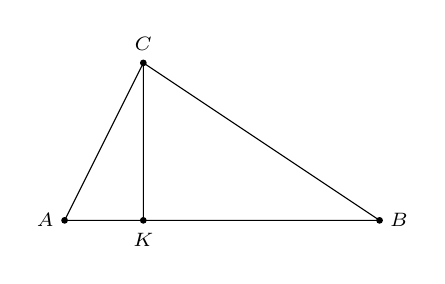
\begin{tikzpicture}
	\path (0,0) coordinate (A)
	(1,2) coordinate (C)
	(4,0)coordinate (B)
	(1,0) coordinate (K)
	;
	\draw (A)--(B)--(C)--cycle (K)--(C);
	\foreach \t/\g in {A/180,C/90,B/0,K/-90}{
	\draw[fill=black] (\t) circle (1pt) node[shift={(\g:7pt)},font=\scriptsize]{$ \t $};
		}	
	\end{tikzpicture}}
}
\end{bt}

\begin{bt}%[0T9B3-2]%[Tex đề GHKI-GHKII K10 NH22-23 đợt 7- Lương Như Quỳnh]%[Trường THPT Nguyễn Trung Trực]
Trong mặt phẳng tọa độ $Oxy$, cho điểm $I(-5;7)$ và đường thẳng $\Delta_1\colon 3x+4y-5=0$.
	\begin{enumerate}
	\item Viết phương trình đường tròn $(C)$ có tâm $I$ và tiếp xúc với đường thẳng $\Delta_1$.
	\item Viết phương trình tiếp tuyến của đường tròn $(C)$ biết tiếp tuyến vuông góc với đường thẳng $\Delta_2\colon x+2 y-1=0$.
	\end{enumerate}
\loigiai{
	\begin{enumerate}
	\item Đường tròn $(C)$ có tâm $I(-5;7)$ và bán kính 
		\[
R=\mathrm{d}(I,\Delta_1)=\dfrac{|3 \cdot (-5)+4 \cdot 7-5|}{\sqrt{3^2+4^2}}=\dfrac{8}{5}.
		\]
		Vậy phương trình đường tròn $(C)\colon (x+5)^2+(y-7)^2=\dfrac{64}{25}$.
		\item Gọi đường thẳng $d$ là tiếp tuyến của $(C)$ vuông góc với đường thẳng $\Delta_2\colon x+2 y-1=0$. \\
			Khi đó, đường thẳng $d$ có phương trình dạng $2x-y+c=0$.\\
			Ta có $$\mathrm{d}(I;d)=R\Leftrightarrow \dfrac{|2\cdot (-5)-7+c|}{\sqrt{2^2+(-1)^2}}=\dfrac{8}{5}\Leftrightarrow|-17+c|=\dfrac{8\sqrt{5}}{5}
			\Leftrightarrow \hoac{&c=\dfrac{85+8\sqrt{5}}{5}\\&c=\dfrac{85-8\sqrt{5}}{5}.}$$
			Vậy $d$ có phương trình $10x-5y+85+8\sqrt{5}=0$ hoặc $10x-5y+85-8\sqrt{5}=0$.
\end{enumerate}		
}
\end{bt}

\begin{bt}%[0T7K2-1]%[Tex đề GHKI-GHKII K10 NH22-23 đợt 7- Lương Như Quỳnh]%[Trường THPT Nguyễn Trung Trực]
Thiết kế của một chiếc cổng có hình parabol với chiều cao $6$ m và khoảng cách giữa hai chân cổng là $4$ m. Người ta cần chuyển một thùng hàng hình hộp chữ nhật với chiều cao $4$ m. Chiều rộng của thùng hàng tối đa là bao nhiêu để thùng có thể chuyển lọt qua được cổng?
	\loigiai{
\immini{
			Chọn hệ trục tọa độ như hình vẽ.\\
			Gọi phương trình của vòm cổng hình parabol là $y=ax^2+bx+c$ ($ a\neq 0 $).\\
			Một chân cổng có tọa độ $(0;0)$ suy ra $c=0$.\quad(1)\\
			Một chân cổng có tọa độ $(4;0)$ suy ra $16a+4b+c=0$. \quad(2)\\
			Đỉnh cổng có tọa độ $(2;6)$ suy ra $4a+2b+c=6$.\quad(3)\\
			Từ $(1)$, $(2)$, $(3)$ ta có hệ phương trình $$\heva{&c=0\\&16a+4b+c=0\\&4a+2b=6} \Leftrightarrow \heva{&a=-1{,}5\\&b=6\\&c=0.}$$
			}
			{
	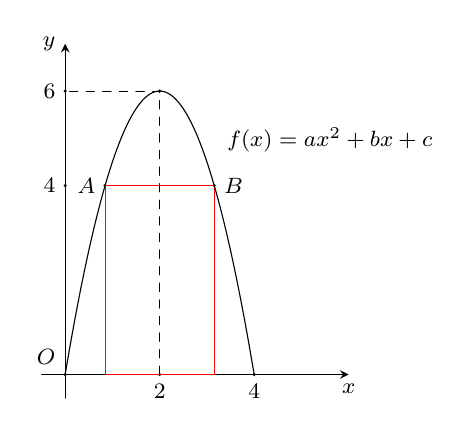
\begin{tikzpicture}[scale=0.6, font=\footnotesize, line join=round, line cap=round, >=stealth]
\def\xmin{-.5} \def\xmax{6}
\def\ymin{-.5} \def\ymax{7} 
\draw[->] (\xmin,0)--(\xmax,0) node [below]{$x$};
\draw[->] (0,\ymin)--(0,\ymax) node [left]{$y$};
\fill (0,0)circle(1pt)node[above left]{$O$} (2,0)circle(1pt)node[below]{$2$} (4,0)circle(1pt)node[below]{$4$}(0,6)circle(1pt)node[left]{$6$}
(0,4)circle(1pt)node[left]{$4$}
(2,6)circle(1pt)
(0.845,4)circle(1pt)node[left]{$A$}
(3.155,4)circle(1pt)node[right]{$B$};
\draw[red] (0.845,0)--(0.845,4)--(3.155,4)--(3.155,0)--cycle;
\draw (5.6,4.5)node[above]{$f(x)=ax^2+bx+c$};
\draw[dashed] (2,0)--(2,6)--(0,6);
\clip (\xmin+0.1,\ymin+0.1) rectangle (\xmax-0.1,\ymax-0.1);
\draw[smooth,samples=300,domain=0:4] plot(\x,{-1.5*\x^2+6*\x});
	\end{tikzpicture}
			}\noindent
			Suy ra phương trình của vòm cổng là $y=-1{,}5x^2+6x$.\\
			Gọi $ A $, $ B $ là hai điểm trên cổng có chiều cao bằng $ 4 $.\\
			Để thùng hàng có thể chuyển lọt qua được cổng thì chiều rộng thùng hàng phải nhỏ hơn $ AB $. \\
			Xét phương trình $-1{,}5x^2+6x = 4\Leftrightarrow -1{,}5x^2+6x-4 =0 \Leftrightarrow \hoac{&x=\dfrac{6-2\sqrt{3}}{3}\\&x= \dfrac{6+2\sqrt{3}}{3}.}$\\
			Suy ra $ x_A=\dfrac{6-2\sqrt{3}}{3} $, $ x_B=\dfrac{6+2\sqrt{3}}{3} $.\\
			Vậy chiều rộng của thùng hàng phải nhỏ hơn \[AB=x_B-x_A=\dfrac{6+2\sqrt{3}}{3}-\dfrac{6-2\sqrt{3}}{3}=\dfrac{4\sqrt{3}}{3} \approx 2{,}3 \text{ m.}\]
}
\end{bt}